\documentclass[12pt,letterpaper]{report}
\usepackage[spanish]{babel}
\usepackage[letterpaper, margin=2.5cm]{geometry}
\usepackage{graphicx}
\usepackage{float}
\usepackage{booktabs}
\usepackage{threeparttable}
\usepackage{tabularx}
\usepackage{longtable}
\usepackage{multirow}
\usepackage{array}
\usepackage{enumitem}
\usepackage{setspace}
\usepackage[hidelinks]{hyperref}
\usepackage{amsmath}
\usepackage{amssymb}
\usepackage{bm}
\usepackage{algorithm}
\usepackage{algpseudocode}
\usepackage{caption}
\usepackage{subcaption}
\usepackage{pdfpages}
\usepackage{nameref}
\usepackage{titlesec}
\usepackage{tikz}
\usetikzlibrary{positioning, arrows.meta, shapes, calc}

% Ajuste de espaciado para títulos de capítulos
% \titlespacing*{<command>}{<left>}{<before-sep>}{<after-sep>}
% before-sep: Espacio antes del título. Por defecto es ~50pt. Aquí lo reducimos.
\titleformat{\chapter}[display]
  {\normalfont\huge\bfseries}{\chaptertitlename\ \thechapter}{20pt}{\Huge}
\titlespacing*{\chapter}{0pt}{0pt}{1pt}

% Configuración de bibliografía - Estilo IEEE
\usepackage[numbers]{natbib}
\bibliographystyle{IEEEtran}

% Nombres en español
\renewcommand{\tablename}{Tabla}
\renewcommand{\figurename}{Figura}
\renewcommand{\contentsname}{Contenido}
\renewcommand{\bibname}{Referencias}
\renewcommand{\listfigurename}{Lista de Figuras}
\renewcommand{\listtablename}{Lista de Tablas}
\renewcommand{\algorithmicforall}{\textbf{para todo}}
\renewcommand{\algorithmicdo}{\textbf{hacer}}
\renewcommand{\algorithmicend}{\textbf{fin}}
\renewcommand{\algorithmicif}{\textbf{si}}
\renewcommand{\algorithmicthen}{\textbf{entonces}}
\renewcommand{\algorithmicelse}{\textbf{sino}}
\renewcommand{\algorithmicwhile}{\textbf{mientras}}
\renewcommand{\algorithmicrepeat}{\textbf{repetir}}
\renewcommand{\algorithmicuntil}{\textbf{hasta que}}
\renewcommand{\algorithmicreturn}{\textbf{devolver}}

% Numeración de ecuaciones, figuras y tablas por capítulo
\numberwithin{equation}{chapter}
\numberwithin{figure}{chapter}
\numberwithin{table}{chapter}

% Evitar hyphenation excesiva
\pretolerance=5000
\tolerance=2000
\emergencystretch=30pt

% BibTeX habilitado - usar natbib con estilo IEEEtran (numérico)

\begin{document}

\setstretch{1.15}

% ============================================================================
% NUMERACIÓN ROMANA PARA PÁGINAS PRELIMINARES
% ============================================================================
\pagenumbering{roman}

% ============================================================================
% PORTADA ORIGINAL (BUAP)
% ============================================================================
\input{portada/title-page}

% ============================================================================
% DEDICATORIA
% ============================================================================
\newpage
\input{dedicatoria/dedicatoria}

% ============================================================================
% AGRADECIMIENTOS
% ============================================================================
\newpage
%----------------------------------------------------------------------------------------
%       AGRADECIMIENTOS
%----------------------------------------------------------------------------------------
\section*{Agradecimientos}
\addcontentsline{toc}{section}{Agradecimientos}

Agradezco a la Secretaría de Ciencia, Humanidades, Tecnología e Innovación (SECIHTI) por el apoyo económico brindado mediante la beca otorgada durante el desarrollo de este trabajo de investigación. Este respaldo fue fundamental para dedicar el tiempo y los recursos necesarios para llevar a cabo esta tesis.

A la Benemérita Universidad Autónoma de Puebla (BUAP), en particular a la Facultad de Ciencias de la Electrónica y al programa de Maestría en Ingeniería Electrónica, Opción Instrumentación Electrónica,  por brindarme la oportunidad de formarme académicamente y proporcionarme las herramientas necesarias para mi desarrollo profesional.

A mis directores de tesis, el Dr. Salvador Eugenio Ayala Raggi y el Dr. Aldrin Barreto Flores, por su invaluable guía, dedicación y paciencia durante todo el proceso de investigación. Sus conocimientos, observaciones críticas y apoyo constante fueron esenciales para la realización de este trabajo.

Al comité revisor conformado por el M.C. Nicolás Quiroz Hernández, la M.C. Ana María Rodríguez Domínguez y la Dra. María Monserrat Morín Castillo, por el tiempo dedicado a la revisión de este trabajo y por sus valiosas observaciones y comentarios, que contribuyeron significativamente a mejorar la calidad de esta tesis.

Finalmente, a mi familia y seres queridos, por su comprensión, apoyo incondicional y motivación constante a lo largo de esta etapa de mi vida académica.


% ============================================================================
% RESUMEN
% ============================================================================
\newpage
% =============================================================================
% RESUMEN / ABSTRACT
% =============================================================================

\section*{Resumen}
\addcontentsline{toc}{section}{Resumen}

La clasificaci\'on autom\'atica de enfermedades pulmonares en radiograf\'ias de t\'orax se enfrenta a un desaf\'io fundamental: la variabilidad de pose, escala y orientación entre im\'agenes. Diferencias en el posicionamiento del paciente, la distancia de proyecci\'on, la fase respiratoria y la calibraci\'on del equipo introducen variaciones que dificultan el aprendizaje de caracter\'isticas patol\'ogicas genuinas por parte de modelos de aprendizaje profundo.

El presente trabajo desarrolla e implementa un sistema de normalizaci\'on geom\'etrica basado en detecci\'on autom\'atica de puntos de referencia anat\'omicos para mejorar la clasificaci\'on de COVID-19, neumon\'ia viral y casos sanos en radiograf\'ias de t\'orax. El sistema integra cuatro componentes: (1) preprocesamiento de contraste mediante CLAHE y SAHS, (2) predicci\'on de 15 puntos de referencia que definen el contorno pulmonar mediante un ensamble de cuatro modelos ResNet-18 con Coordinate Attention y aumento en tiempo de prueba, (3) normalizaci\'on geom\'etrica mediante An\'alisis Procrustes Generalizado para c\'alculo de forma est\'andar, triangulaci\'on de Delaunay y deformaci\'on af\'in por partes, y (4) clasificaci\'on mediante una red neuronal convolucional entrenada sobre las im\'agenes normalizadas geométricamente.

El modelo de detecci\'on de puntos de referencia alcanza un error promedio de 3.61 p\'ixeles en im\'agenes de 224$\times$224 p\'ixeles, equivalente al 1.61\% de la diagonal de la imagen, con una mejora del 10.6\% respecto al mejor modelo individual mediante la estrategia de ensamble. El clasificador entrenado sobre im\'agenes normalizadas geom\'etricamente obtiene una exactitud de 98.60\% y un F1-Score Macro de 98.00\% mediante validaci\'on cruzada de cinco pliegues sobre un conjunto de prueba de 1,895 im\'agenes.

La contribuci\'on principal es la validaci\'on experimental de que la normalizaci\'on geom\'etrica mejora la clasificaci\'on al reducir la variabilidad de pose, escala y orientación. Un experimento comparativo de cuatro configuraciones de preprocesamiento proporciona evidencia directa: al eliminar los bordes de las im\'agenes originales mediante recorte simple, la exactitud cae de 98.68\% a 95.36\% ($-$3.32 puntos porcentuales), demostrando que los modelos entrenados sin normalizaci\'on geométrica dependen de artefactos hospitalarios. El sistema propuesto recupera este rendimiento (98.60\%) utilizando exclusivamente la regi\'on pulmonar normalizada, lo que confirma que la normalizaci\'on geom\'etrica permite al clasificador aprender caracter\'isticas cl\'inicamente relevantes. Esta mejora se valida adicionalmente con un clasificador tradicional basado en PCA, proyecci\'on discriminante de Fisher y KNN, que obtiene $+$3.38 puntos porcentuales con im\'agenes normalizadas, confirmando que el beneficio de la normalizaci\'on geom\'etrica no es espec\'ifico de arquitecturas de aprendizaje profundo sino que mejora la separabilidad entre clases de forma general.

\textbf{Palabras clave:} normalizaci\'on geom\'etrica, puntos de referencia anat\'omicos, radiograf\'ias de t\'orax, COVID-19, deformaci\'on af\'in por partes, An\'alisis Procrustes Generalizado, aprendizaje profundo.

\vspace{1.5cm}


% ============================================================================
% ABSTRACT (INGLÉS)
% ============================================================================
\newpage
% =============================================================================
% ABSTRACT (INGLÉS)
% =============================================================================

\section*{Abstract}
\addcontentsline{toc}{section}{Abstract}

The automatic classification of pulmonary diseases in chest radiographs faces a fundamental challenge: variability in pose, scale, and orientation between images. Differences in patient positioning, projection distance, respiratory phase, and equipment calibration introduce variations that hinder the learning of genuine pathological features by deep learning models.

This work develops and implements a geometric normalization system based on automatic detection of anatomical landmarks to improve the classification of COVID-19, viral pneumonia, and healthy cases in chest radiographs. The system integrates four components: (1) contrast preprocessing using CLAHE and SAHS, (2) prediction of 15 landmarks defining the lung contour through an ensemble of four ResNet-18 models with Coordinate Attention and test-time augmentation, (3) geometric normalization via Generalized Procrustes Analysis for standard shape computation, Delaunay triangulation, and piecewise affine deformation, and (4) classification through a convolutional neural network trained on geometrically normalized images.

The landmark detection model achieves an average error of 3.61 pixels on 224$\times$224 pixel images, equivalent to 1.61\% of the image diagonal, with a 10.6\% improvement over the best individual model through the ensemble strategy. The classifier trained on geometrically normalized images obtains 98.60\% accuracy and 98.00\% Macro F1-Score through five-fold cross-validation on a test set of 1,895 images.

The main contribution is the experimental validation that geometric normalization improves classification by reducing pose, scale, and orientation variability. A comparative experiment of four preprocessing configurations provides direct evidence: when eliminating borders from original images through simple cropping, accuracy drops from 98.68\% to 95.36\% ($-$3.32 percentage points), demonstrating that models trained without geometric normalization depend on hospital artifacts. The proposed system recovers this performance (98.60\%) using exclusively the normalized lung region, confirming that geometric normalization allows the classifier to learn clinically relevant features. This improvement is additionally validated with a traditional classifier based on PCA, Fisher discriminant projection, and KNN, which obtains $+$3.38 percentage points with normalized images, confirming that the benefit of geometric normalization is not specific to deep learning architectures but improves class separability in general.

\textbf{Keywords:} geometric normalization, anatomical landmarks, chest radiographs, COVID-19, piecewise affine deformation, Generalized Procrustes Analysis, deep learning.

\vspace{1.5cm}


% ============================================================================
% TABLA DE CONTENIDO
% ============================================================================
\newpage
\tableofcontents

% ============================================================================
% LISTA DE FIGURAS
% ============================================================================
\newpage
\addcontentsline{toc}{section}{Lista de Figuras}
\listoffigures

% ============================================================================
% LISTA DE TABLAS
% ============================================================================
\newpage
\addcontentsline{toc}{section}{Lista de Tablas}
\listoftables

% ============================================================================
% NUMERACIÓN ARÁBIGA PARA CAPÍTULOS
% ============================================================================
\newpage
\pagenumbering{arabic}

% ============================================================================
% CAPÍTULO 1: INTRODUCCIÓN
% ============================================================================
\input{capitulo1/1_introduccion}

% ============================================================================
% OBJETIVOS (Dentro del Capítulo 1)
% ============================================================================
\input{objetivos/0-Objetivos}

% ============================================================================
% CAPÍTULO 2: MARCO TEÓRICO
% ============================================================================
\newpage
\input{capitulo2/2_marco_teorico}

% ============================================================================
% CAPÍTULO 3: ESTADO DEL ARTE
% ============================================================================
\newpage
\input{capitulo3/3_estado_del_arte}

% ============================================================================
% CAPÍTULO 4: METODOLOGÍA
% ============================================================================
\newpage

% Sección 4.1: Descripción General del Sistema
\input{capitulo4/4_1_descripcion_general}

% Sección 4.2: Dataset y Preprocesamiento
\newpage
\input{capitulo4/4_2_dataset_preprocesamiento}

% Sección 4.3: Modelo de Predicción de Landmarks
\newpage
\input{capitulo4/4_3_modelo_landmarks}

% Sección 4.4: Normalización Geométrica
\newpage
\input{capitulo4/4_4_normalizacion_geometrica}

% Sección 4.5: Clasificación de Enfermedades Pulmonares
\newpage
\input{capitulo4/4_5_clasificacion}

% Sección 4.6: Protocolo de Inferencia y Evaluación
\newpage
\input{capitulo4/4_6_inferencia_metricas}

% ============================================================================
% CAPÍTULO 5: RESULTADOS
% ============================================================================
\newpage

% Sección 5.1: Detección de Puntos de Referencia (incluye \chapter{Resultados})
\input{capitulo5/5_1_resultados_landmarks}

% Sección 5.2: Normalización Geométrica
\newpage
\input{capitulo5/5_2_forma_canonica}

% Sección 5.3: Clasificación de Enfermedades Pulmonares
\newpage
\input{capitulo5/5_3_resultados_clasificacion}

% Sección 5.4: Eficiencia Computacional
\newpage
% =============================================================================
% CAPÍTULO 5: RESULTADOS
% Sección 5.4: Eficiencia Computacional
% =============================================================================

\section{Eficiencia Computacional}
\label{sec:eficiencia_computacional}

Esta sección analiza los tiempos de inferencia del sistema medidos sobre 100 imágenes del conjunto de prueba en el hardware descrito en la Sección \ref{subsec:hardware_specs}.

\subsection{Tiempos de Inferencia}
\label{subsec:tiempos_inferencia}

La Tabla \ref{tab:tiempos_inferencia} presenta los tiempos medidos para cada módulo del proceso.

\begin{table}[htbp]
    \centering
    \caption{Tiempos de inferencia por módulo (ms). Estadísticas sobre 100 imágenes.}
    \label{tab:tiempos_inferencia}
    \small
    \begin{tabular}{@{}lcccc@{}}
        \toprule
        \textbf{Módulo} & \textbf{Media} & \textbf{Mediana} & \textbf{Desv. Std.} & \textbf{\% Total} \\
        \midrule
        Preprocesamiento CLAHE & 0.45 & 0.18 & 0.56 & 0.5\% \\
        Puntos de Referencia (Ensamble + TTA) & 66.08 & 59.34 & 14.64 & 73.5\% \\
        Normalización Geométrica & 4.86 & 4.26 & 1.22 & 5.4\% \\
        Preprocesamiento SAHS & 0.53 & 0.51 & 0.13 & 0.6\% \\
        Clasificación & 8.59 & 6.90 & 3.40 & 9.6\% \\
        \midrule
        \textbf{Proceso Completo} & \textbf{89.92} & \textbf{79.24} & \textbf{20.31} & \textbf{100\%} \\
        \bottomrule
    \end{tabular}
\end{table}

El sistema procesa una imagen completa en \textbf{89.92 ms promedio} (\textbf{11.1 imágenes/segundo}). El módulo de ensamble de puntos de referencia es el cuello de botella, representando el 73.5\% del tiempo total, mientras que el preprocesamiento ($<$1\%) y warping (5.4\%) tienen impacto mínimo.


% ============================================================================
% CAPÍTULO 6: CONCLUSIONES Y TRABAJOS FUTUROS
% ============================================================================
\newpage
\input{capitulo6/6_conclusiones}

% ============================================================================
% REFERENCIAS
% ============================================================================
\newpage
\bibliography{references}

% ============================================================================
% ANEXOS
% ============================================================================
\appendix
\newpage
% TEMPORAL: Comentado para revisión posterior (Sesión 6)
% El Anexo A (Manual de Usuario de la GUI) requiere revisión adicional
% antes de su inclusión definitiva en la tesis
%%----------------------------------------------------------------------------------------
%       ANEXO A: MANUAL DE USUARIO
%----------------------------------------------------------------------------------------
\chapter{Manual de Usuario - Interfaz Gráfica de Demostración}
\label{anexo:manual_usuario}

Este anexo presenta el manual de usuario de la interfaz gráfica desarrollada para demostrar el sistema completo de detección de COVID-19 mediante landmarks anatómicos y normalización geométrica.

\section{Descripción General}

La interfaz gráfica está implementada con Gradio, un framework para crear interfaces web interactivas en Python. El sistema permite visualizar las cuatro etapas principales del pipeline de procesamiento:

\begin{enumerate}
    \item Imagen original de radiografía de tórax
    \item Detección de 15 landmarks anatómicos
    \item Imagen normalizada mediante warping geométrico
    \item Mapa de atención GradCAM mostrando regiones relevantes para la clasificación
\end{enumerate}

\section{Requisitos del Sistema}

\subsection{Dependencias de Software}

\begin{itemize}
    \item Python 3.8 o superior
    \item Gradio 4.0.0 o superior
    \item PyTorch con soporte para GPU (opcional, recomendado)
    \item Dependencias adicionales especificadas en \texttt{requirements.txt}
\end{itemize}

\subsection{Modelos Necesarios}

El sistema requiere los siguientes archivos de modelos entrenados:

\textbf{Ensemble de Landmarks (4 modelos):}
\begin{itemize}
    \item \texttt{checkpoints/session10/ensemble/seed123/final\_model.pt}
    \item \texttt{checkpoints/session13/seed321/final\_model.pt}
    \item \texttt{checkpoints/repro\_split111/session14/seed111/final\_model.pt}
    \item \texttt{checkpoints/repro\_split666/session16/seed666/final\_model.pt}
\end{itemize}

\textbf{Forma Canónica y Triangulación:}
\begin{itemize}
    \item \texttt{outputs/shape\_analysis/canonical\_shape\_gpa.json}
    \item \texttt{outputs/shape\_analysis/canonical\_delaunay\_triangles.json}
\end{itemize}

\textbf{Clasificador:}
\begin{itemize}
    \item {\small \texttt{outputs/classifier\_warped\_lung\_best/sweeps\_2026-01-12/\linebreak lr2e-4\_seed321\_on/best\_classifier.pt}}
\end{itemize}

\section{Instalación y Ejecución}

\subsection{Lanzar la Interfaz}

Existen dos opciones para ejecutar la interfaz:

\paragraph{Opción 1 (Recomendada):} Usar el script de lanzamiento con verificaciones automáticas:

\begin{verbatim}
python scripts/run_demo.py
\end{verbatim}

Opciones disponibles:
\begin{itemize}
    \item \texttt{-{}-share}: Crear enlace público compartible
    \item \texttt{-{}-port PORT}: Cambiar puerto (predeterminado: 7860)
    \item \texttt{-{}-host HOST}: Cambiar host (predeterminado: localhost)
\end{itemize}

\paragraph{Opción 2:} Ejecutar directamente el módulo:

\begin{verbatim}
python -m src_v2.gui.app
\end{verbatim}

La interfaz se abrirá automáticamente en el navegador web en \texttt{http://localhost:7860}.

\section{Uso de la Interfaz}

\subsection{Tab 1: Demostración Completa}

Esta pestaña muestra el pipeline completo con visualizaciones de todas las etapas:

\begin{enumerate}
    \item \textbf{Cargar imagen:}
    \begin{itemize}
        \item Arrastrar y soltar una radiografía de tórax en el área designada
        \item Hacer clic en el botón de carga para seleccionar un archivo
        \item Seleccionar uno de los ejemplos precargados (COVID, Normal, Viral)
    \end{itemize}

    \item \textbf{Procesar:}
    \begin{itemize}
        \item Hacer clic en el botón ``Procesar Imagen''
        \item Esperar 1-2 segundos mientras el sistema procesa (el tiempo varía según el hardware)
    \end{itemize}

    \item \textbf{Visualizar resultados:}
    \begin{itemize}
        \item La interfaz mostrará 4 imágenes correspondientes a cada etapa del pipeline
        \item Se mostrarán las probabilidades de clasificación para cada clase
        \item Es posible expandir la sección ``Métricas Detalladas'' para ver el error promedio por landmark
    \end{itemize}

    \item \textbf{Exportar (opcional):}
    \begin{itemize}
        \item Hacer clic en ``Exportar Resultados a PDF''
        \item El sistema generará un reporte PDF con todas las visualizaciones y métricas
        \item El archivo se guardará en el directorio de trabajo actual
    \end{itemize}
\end{enumerate}

\subsection{Tab 2: Vista Rápida}

Esta pestaña proporciona una clasificación directa sin visualizaciones intermedias:

\begin{enumerate}
    \item Cargar la radiografía de tórax
    \item Hacer clic en ``Clasificar''
    \item Obtener el resultado inmediato (clase predicha y probabilidades)
\end{enumerate}

Esta opción es útil cuando se requiere únicamente la clasificación sin inspeccionar las etapas intermedias.

\subsection{Tab 3: Acerca del Sistema}

Esta pestaña contiene información sobre:
\begin{itemize}
    \item Metodología de landmarks y normalización geométrica
    \item Arquitectura del sistema
    \item Métricas validadas del modelo
    \item Referencias bibliográficas
\end{itemize}

\section{Visualización de Landmarks}

Los 15 landmarks se visualizan con un código de colores según su grupo anatómico:

\begin{table}[H]
\centering
\begin{tabular}{llp{6cm}}
\toprule
\textbf{Grupo} & \textbf{Landmarks} & \textbf{Descripción} \\
\midrule
Eje & L1, L2 & Puntos superior e inferior del eje central \\
Central & L9, L10, L11 & Puntos intermedios del eje central \\
Lateral & L3--L8 & Contornos laterales izquierdo y derecho \\
Borde & L12, L13 & Puntos de borde superior \\
Costal & L14, L15 & Puntos costales inferiores \\
\bottomrule
\end{tabular}
\caption{Grupos de landmarks y su representación visual}
\end{table}

\section{Métricas del Sistema}

Las métricas validadas que se muestran en la interfaz son:

\begin{table}[H]
\centering
\begin{tabular}{lc}
\toprule
\textbf{Métrica} & \textbf{Valor} \\
\midrule
Error de Landmarks (píxeles) & $3.61 \pm 2.48$ \\
Accuracy de Clasificación & 98.05\% \\
F1-Score Macro & 97.12\% \\
F1-Score Weighted & 98.04\% \\
\bottomrule
\end{tabular}
\caption{Métricas validadas del sistema completo}
\end{table}

Estos valores fueron obtenidos mediante evaluación rigurosa en el conjunto de prueba y están documentados en el archivo \texttt{GROUND\_TRUTH.json} versión 2.1.0.

\section{Solución de Problemas}

\subsection{Error: Modelos no encontrados}

Si la interfaz reporta que no encuentra los modelos:
\begin{itemize}
    \item Verificar que los archivos de checkpoints existen en las rutas especificadas
    \item Ejecutar \texttt{python scripts/run\_demo.py} para diagnóstico automático
    \item Consultar la documentación de reproducción del pipeline completo
\end{itemize}

\subsection{Error: Memoria GPU insuficiente}

La interfaz automáticamente detectará problemas de memoria GPU y realizará fallback a CPU:
\begin{itemize}
    \item El tiempo de inferencia será aproximadamente 2-3× más lento en CPU
    \item Para forzar el uso de CPU, modificar \texttt{DEVICE\_PREFERENCE = "cpu"} en \texttt{config.py}
\end{itemize}

\subsection{La interfaz no se abre en el navegador}

\begin{itemize}
    \item Verificar que el puerto 7860 no esté siendo utilizado por otra aplicación
    \item Usar la opción \texttt{-{}-port 8080} para cambiar el puerto
    \item Revisar la configuración del firewall si se usa la opción \texttt{-{}-share}
\end{itemize}

\subsection{Imágenes de baja calidad}

\begin{itemize}
    \item Tamaño mínimo recomendado: 100×100 píxeles
    \item Tamaño óptimo: 224×224 píxeles o superior
    \item La interfaz redimensiona automáticamente las imágenes al tamaño requerido
\end{itemize}

\section{Arquitectura del Sistema}

\subsection{Patrón Singleton para Gestión de Modelos}

El módulo \texttt{ModelManager} utiliza el patrón Singleton para optimizar el uso de memoria:
\begin{itemize}
    \item \textbf{Lazy loading}: Los modelos se cargan únicamente cuando se utilizan por primera vez
    \item \textbf{Cacheo en memoria}: Los modelos permanecen en memoria entre inferencias
    \item \textbf{Detección automática}: El sistema detecta automáticamente si hay GPU disponible
\end{itemize}

\subsection{Pipeline de Inferencia}

El flujo de procesamiento sigue las siguientes etapas:

\begin{enumerate}
    \item \textbf{Validación}: Verificar formato y dimensiones de la imagen
    \item \textbf{Preprocesamiento}: Cargar y redimensionar a 224×224 píxeles
    \item \textbf{Predicción de landmarks}:
    \begin{itemize}
        \item Aplicar CLAHE (clip=2.0, tile\_size=4)
        \item Ejecutar ensemble de 4 modelos
        \item Aplicar TTA (Test-Time Augmentation) con flip horizontal
        \item Promediar predicciones para obtener landmarks finales (15, 2)
    \end{itemize}
    \item \textbf{Warping}: Normalización geométrica mediante transformación afín por piezas
    \item \textbf{Clasificación}: Inferencia con ResNet-18 y generación de GradCAM
    \item \textbf{Visualización}: Renderizado de las 4 etapas para presentación al usuario
\end{enumerate}

\section{Notas Técnicas}

\subsection{Formato de Imágenes Soportadas}

La interfaz acepta los siguientes formatos:
\begin{itemize}
    \item PNG (.png)
    \item JPEG (.jpg, .jpeg)
    \item Escala de grises o RGB (se convierte automáticamente a escala de grises)
\end{itemize}

\subsection{Tiempo de Procesamiento}

El tiempo de procesamiento típico es:
\begin{itemize}
    \item Con GPU (NVIDIA con CUDA): 1-2 segundos
    \item Con CPU (multi-core moderno): 3-5 segundos
    \item El primer procesamiento puede tardar más debido a la carga inicial de modelos
\end{itemize}

\subsection{Uso de Recursos}

\begin{itemize}
    \item Memoria GPU requerida: $\sim$2 GB
    \item Memoria RAM requerida: $\sim$4 GB
    \item Espacio en disco para modelos: $\sim$500 MB
\end{itemize}


\newpage
%----------------------------------------------------------------------------------------
%       ANEXO B: ARTÍCULOS PUBLICADOS
%----------------------------------------------------------------------------------------
\chapter{Artículos Publicados}
\label{anexo:articulos_publicados}

Este anexo presenta los artículos científicos publicados como resultado de la investigación realizada en esta tesis. Los trabajos fueron publicados en revistas arbitradas con registro ISSN y abordan el método de mejora de contraste mediante expansión estadística asimétrica de histograma (SAHS), una técnica de preprocesamiento complementaria a la normalización geométrica desarrollada en este trabajo.

\section{Artículo en Revista Internacional (Inglés)}

El siguiente artículo fue publicado en una revista científica internacional arbitrada. El trabajo describe el método SAHS (Statistical Asymmetrical Histogram Stretching) para mejora de contraste en imágenes de rayos X de tórax, el cual se combina con un algoritmo localizador de pulmones (ALP) para mejorar la detección de neumonía utilizando redes neuronales convolucionales.

\textbf{Título:} Statistical Asymmetrical Histogram Stretching for Contrast Enhancement in Chest X-ray Images for Pneumonia Detection

\textbf{Autores:} Rafael Alejandro Cruz Ovando\textsuperscript{1}, Salvador E. Ayala Raggi\textsuperscript{1}, Ángel E. Picazo Castillo\textsuperscript{2}, Aldrin Barreto Flores\textsuperscript{1}, José Francisco Portillo Robledo\textsuperscript{1}

\textbf{Afiliaciones:}
\begin{enumerate}
\item Benemérita Universidad Autónoma de Puebla, México
\item Instituto Nacional de Astrofísica, Óptica y Electrónica (INAOE), México
\end{enumerate}

\textbf{Revista:} Computación y Sistemas, Vol. 29, No. 4, 2025, pp. 2211–2222

\textbf{DOI:} 10.13053/CyS-29-4-6115

\textbf{ISSN:} 2007-9737

\textbf{Fechas:} Recibido: 01/06/2025, Aceptado: 02/10/2025

\textbf{Resumen:} Este artículo presenta un enfoque para mejorar el contraste en imágenes de rayos X de tórax mediante la técnica SAHS, que aborda la asimetría inherente en los histogramas de este tipo de imágenes. El método se evalúa en diversas arquitecturas CNN (AlexNet, Compact, Enhanced, ResNet-18, MobileNetV2, ResNet-50) y demuestra mejoras consistentes en la precisión de clasificación de neumonía, particularmente en la preservación de regiones brillantes diagnósticamente relevantes.

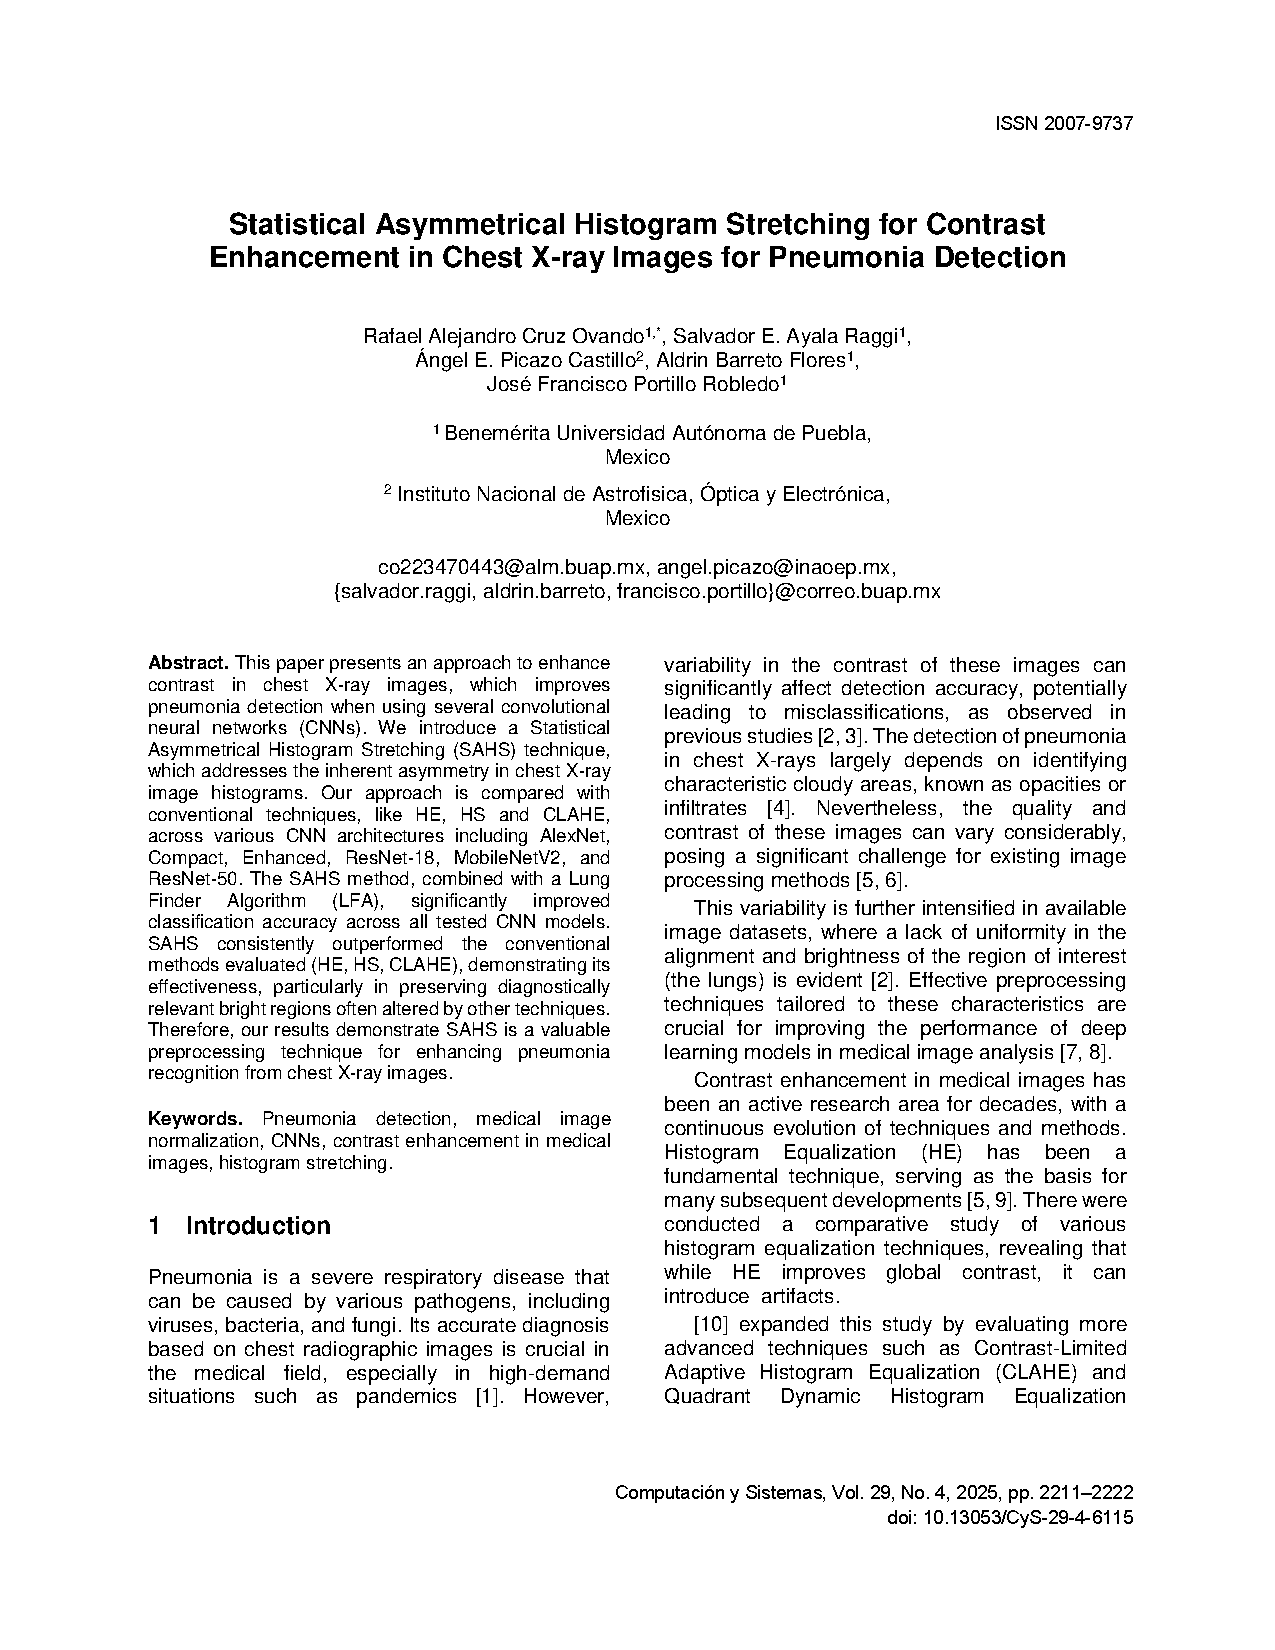
\includepdf[pages=-,pagecommand={\thispagestyle{plain}}]{anexos/articulo_ingles_sahs_2024.pdf}

\section{Artículo en Revista Nacional (Español)}

El siguiente artículo corresponde a la versión en español del trabajo anterior, publicado en una revista científica nacional.

\textbf{Título:} Enfoque de expansión estadística de histograma asimétrico para mejorar el contraste en imágenes de radiografías de tórax para la detección de neumonía

\textbf{Autores:} Rafael Alejandro Cruz Ovando\textsuperscript{1}, Salvador E. Ayala Raggi\textsuperscript{1}, Ángel E. Picazo Castillo\textsuperscript{2}, Aldrin Barreto Flores\textsuperscript{1}, José Francisco Portillo Robledo\textsuperscript{1}

\textbf{Afiliaciones:}
\begin{enumerate}
\item Benemérita Universidad Autónoma de Puebla, Av. San Claudio s/n, Cd Universitaria, C.P. 72592, Puebla, Puebla, México
\item Instituto Nacional de Astrofísica, Óptica y Electrónica, Luis Enrique Erro \#1, C.P. 72840, Sta. María Tonantzintla, Puebla, México
\end{enumerate}

\textbf{Revista:} Abstraction \& Application, Vol. 48, 2024, pp. 133–143

\textbf{Clasificación:} 2020 Mathematics Subject Classification: 68N01

\textbf{Palabras clave:} Detección de Neumonía, Normalización de Imágenes Médicas, CNNs, Mejora de Contraste en Imágenes Médicas, Expansión de Histograma

\textbf{Fechas:} Recibido: 5 de agosto, 2024; Aceptado: 7 de octubre, 2024

\textbf{Resumen:} Este trabajo presenta la técnica SAHS (Statistical Asymmetrical Histogram Stretching) para mejorar el contraste en imágenes de radiografías de tórax, abordando la asimetría inherente en los histogramas de este tipo de imágenes. El método se compara con técnicas convencionales (HE, CLAHE) en diversas arquitecturas CNN, demostrando su eficacia en preservar información crítica como regiones brillantes que indican neumonía. Los resultados muestran que SAHS supera consistentemente a CLAHE en la mayoría de los casos evaluados.

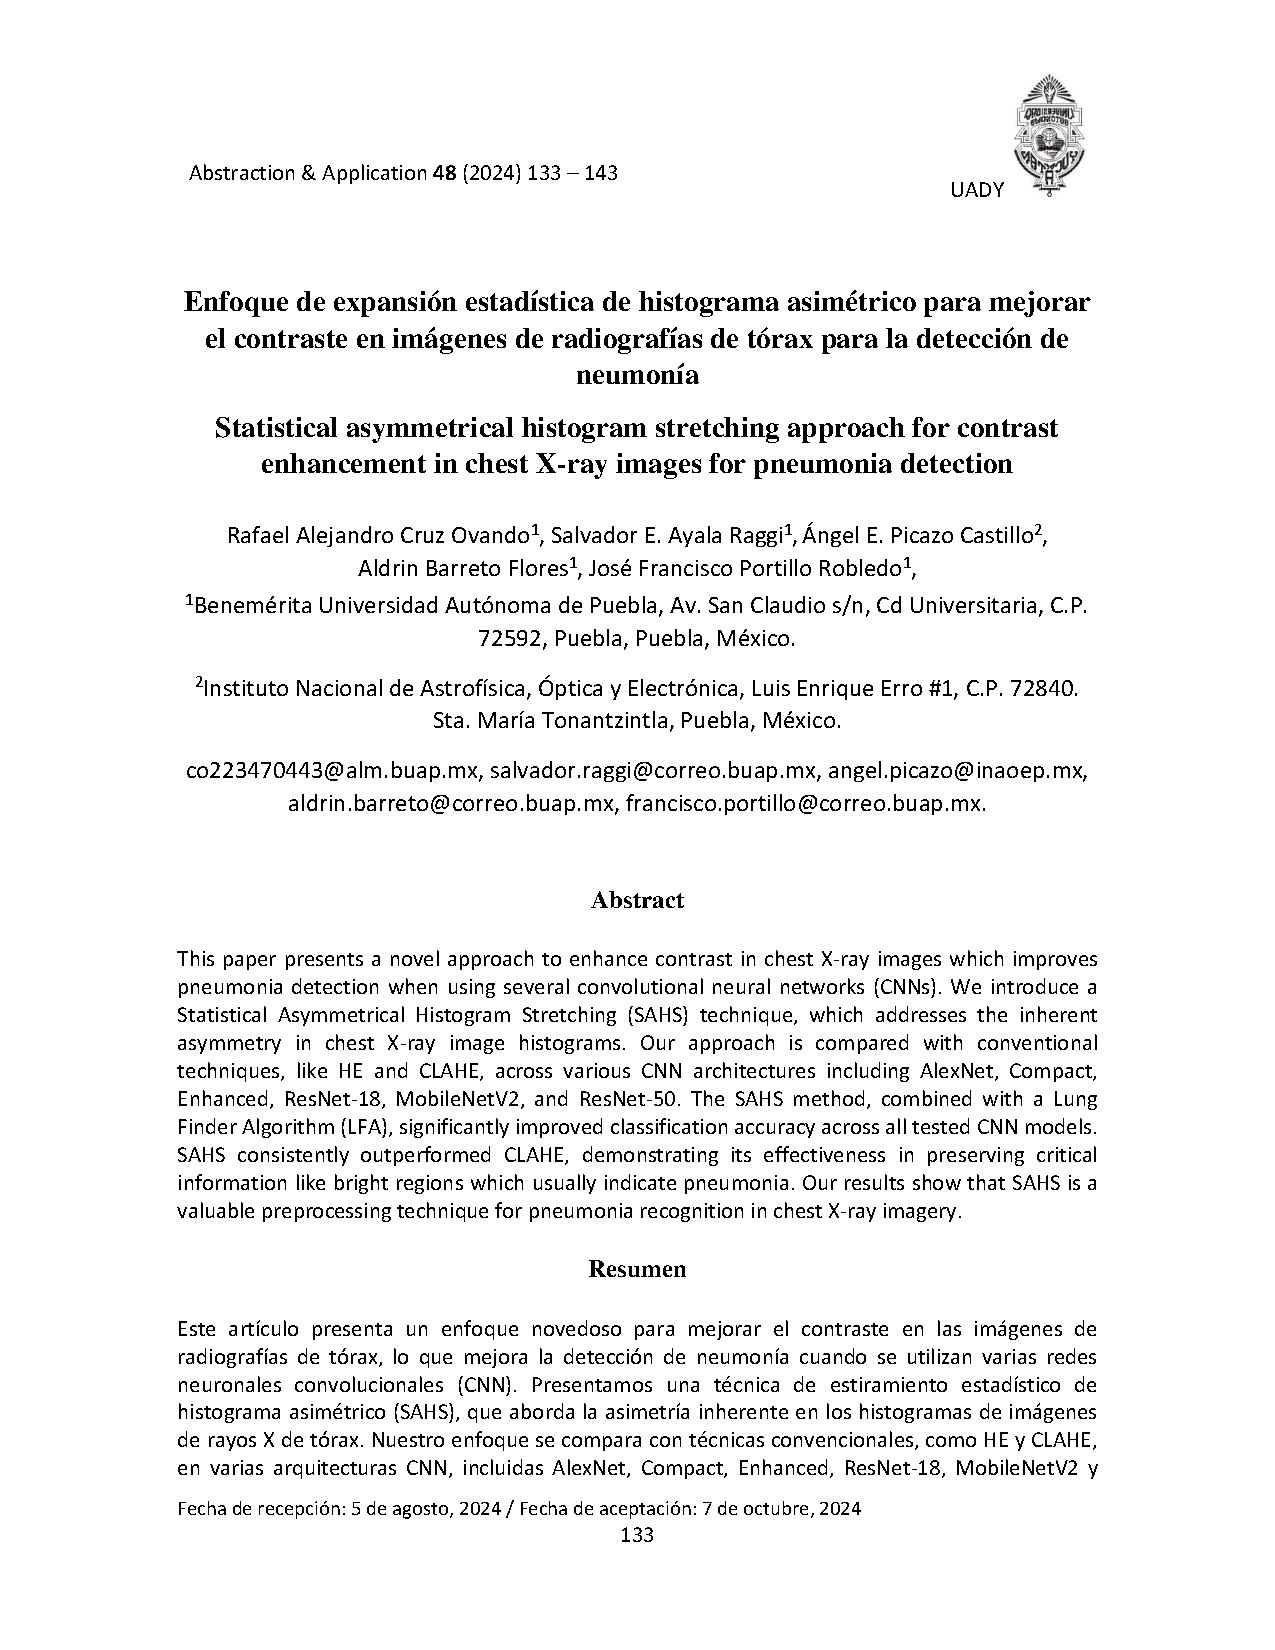
\includepdf[pages=-,pagecommand={\thispagestyle{plain}}]{anexos/articulo_espanol_sahs_2024.pdf}


\newpage
%----------------------------------------------------------------------------------------
%       ANEXO C: CERTIFICADOS Y RECONOCIMIENTOS
%----------------------------------------------------------------------------------------
\chapter{Certificados y Reconocimientos}
\label{anexo:certificados}

Este anexo presenta los certificados, reconocimientos y constancias de participación obtenidos durante el desarrollo de esta investigación. Estos documentos dan testimonio de la difusión de los resultados en congresos, jornadas académicas y eventos científicos organizados por instituciones nacionales e internacionales, así como de actividades de divulgación relacionadas con visión por computadora y aprendizaje profundo.

\section{Reconocimiento - Encuentro NOVA}

\textbf{Evento:} Encuentro de Jóvenes Investigadores NOVA (Evento INSIGNIA NOVA)

\textbf{Fecha:} 12 y 13 de noviembre de 2025

\textbf{Lugar:} Auditorio de la Facultad de Ciencias de la Electrónica, Benemérita Universidad Autónoma de Puebla

\textbf{Institución organizadora:} Rama Estudiantil IEEE BUAP

\textbf{Tipo de participación:} Presentación de poster científico

\textbf{Título del trabajo presentado:} ``Normalización y alineación automática de la forma de la región pulmonar integrada con selección de características discriminantes para detección de neumonía y COVID-19''

\textbf{Descripción:} Este reconocimiento se otorga por la presentación de un poster científico en el Encuentro NOVA, donde se expuso la metodología de normalización geométrica mediante landmarks y warping piecewise affine para la detección de neumonía y COVID-19. Este trabajo está directamente relacionado con la investigación central de esta tesis.

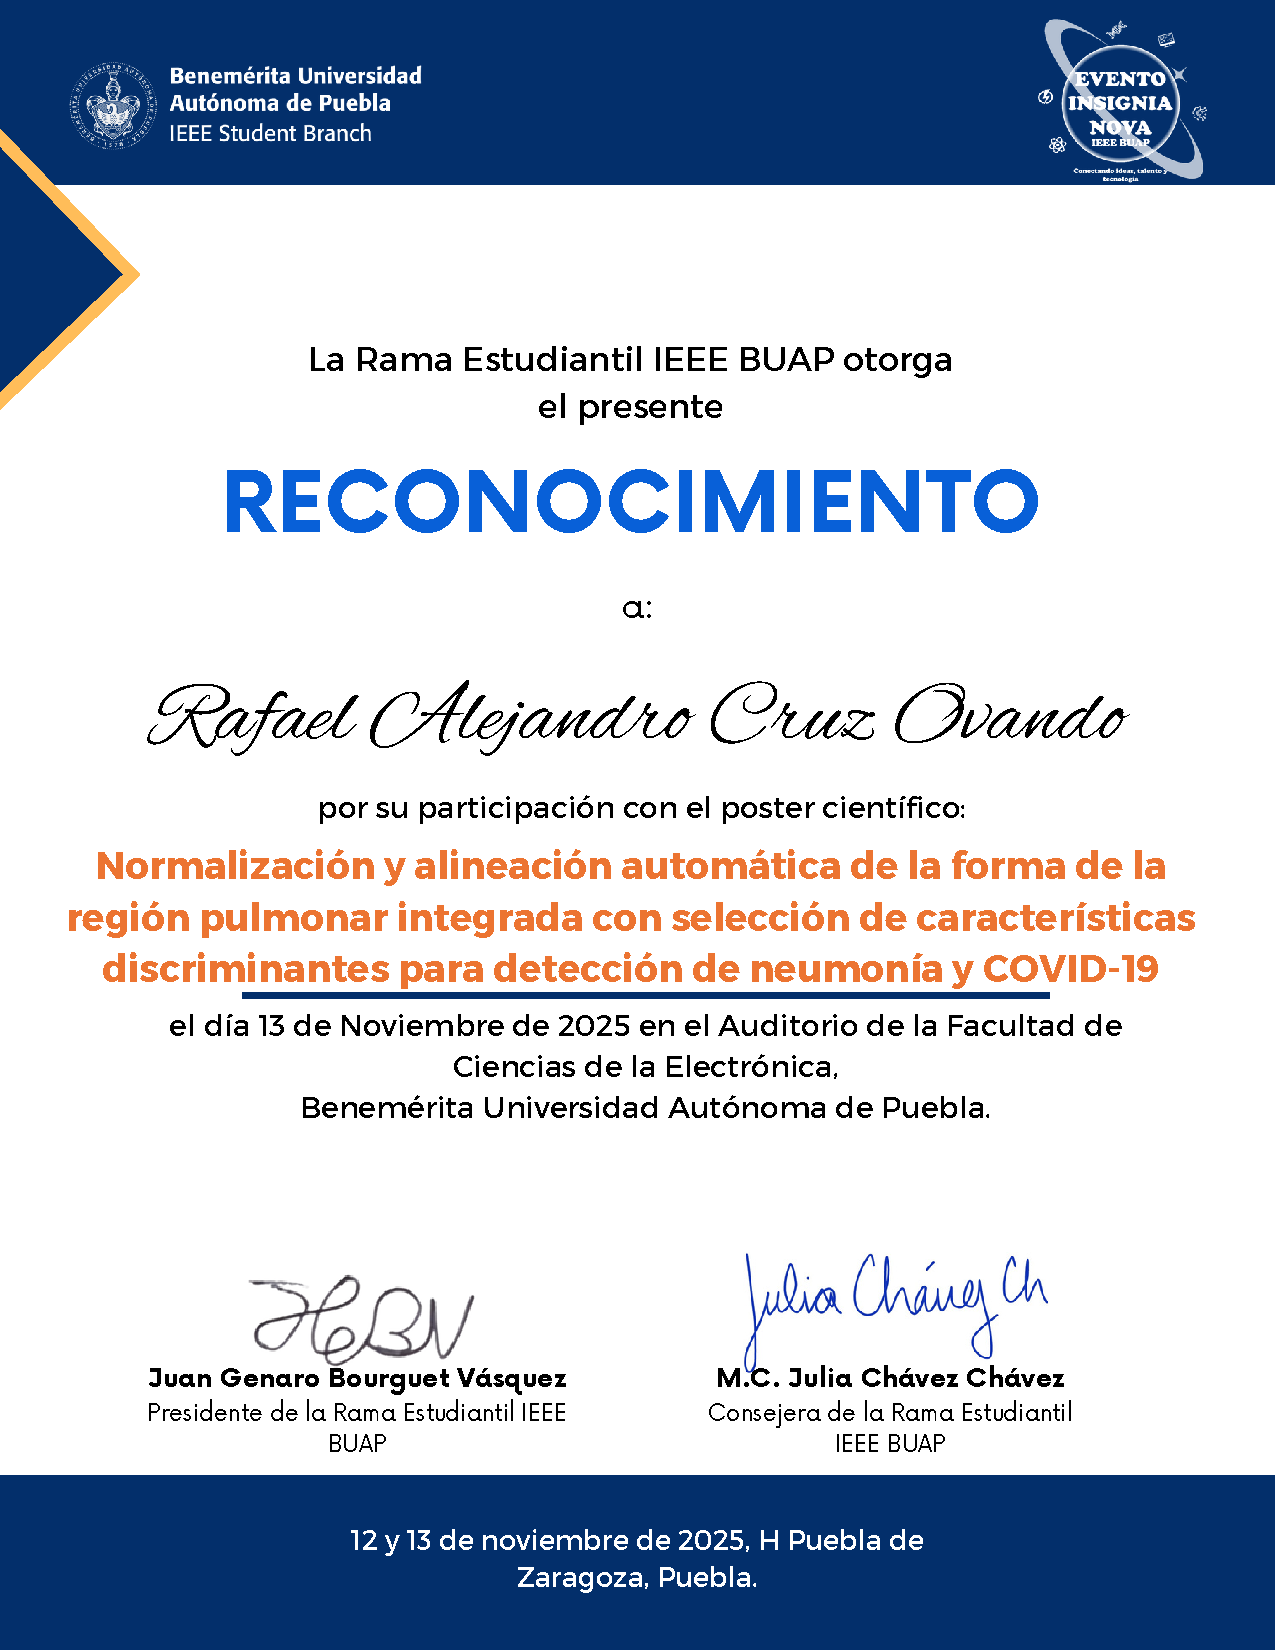
\includepdf[pages=-,pagecommand={\thispagestyle{plain}}]{anexos/reconocimiento_nova.pdf}

\section{Reconocimiento - IEEE DAY}

\textbf{Evento:} IEEE DAY

\textbf{Fecha:} 15 de octubre de 2025

\textbf{Institución organizadora:} IEEE Capítulo Estudiantil BUAP

\textbf{Tipo de participación:} Presentación técnica

\textbf{Título de la presentación:} ``Introducción a Redes Neuronales''

\textbf{Descripción:} Este certificado se otorga por la presentación técnica sobre fundamentos de redes neuronales en el evento IEEE DAY, organizado por la Rama Estudiantil IEEE de la Facultad de Ciencias de la Electrónica, BUAP. La presentación abordó conceptos fundamentales de redes neuronales, tema relacionado con las arquitecturas CNN utilizadas en el clasificador de esta tesis.

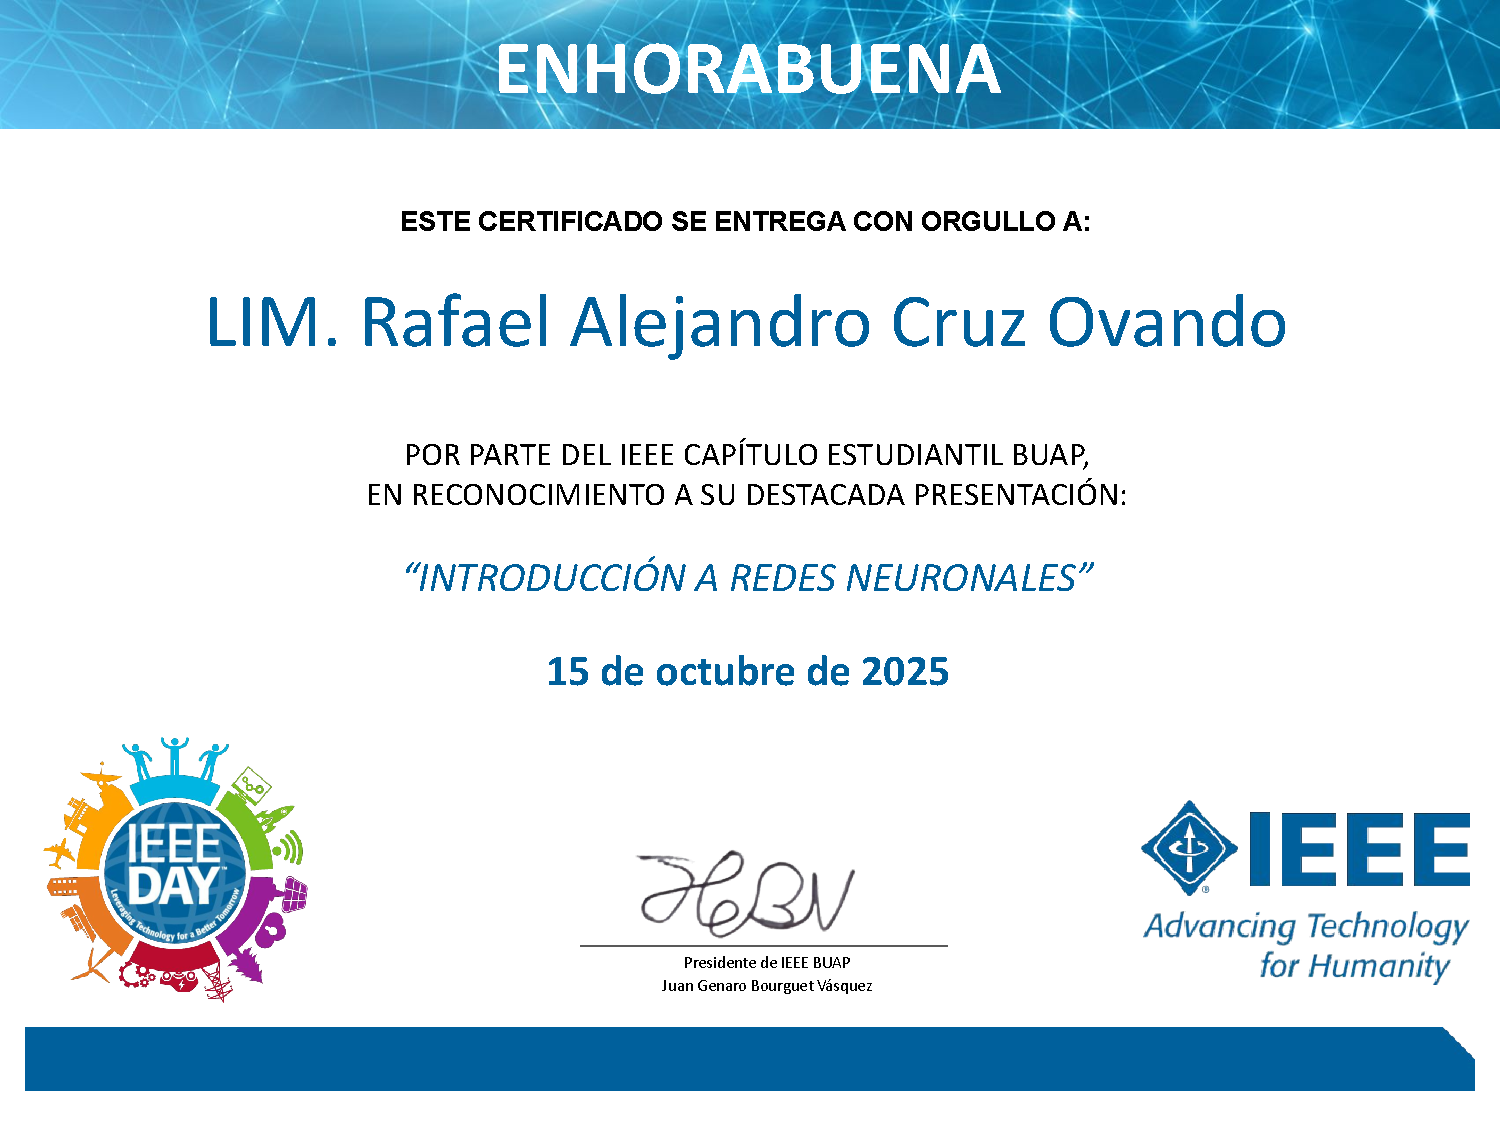
\includepdf[pages=-,pagecommand={\thispagestyle{plain}}]{anexos/reconocimiento_ieee_day.pdf}

\section{Constancia de Participación - RVP-AI ROC\&C 2025 y Congreso de Estudiantes IEEE}

\textbf{Evento principal:} RVP-AI ROC\&C 2025)

\textbf{Evento asociado:} Congreso de Estudiantes IEEE (28 y 29 de julio de 2025)

\textbf{Fecha:} 27 al 31 de julio de 2025

\textbf{Lugar:} Palacio Mundo Imperial, Riviera Diamante, Acapulco, Guerrero

\textbf{Institución organizadora:} IEEE Sección México

\textbf{Firmante:} Dr. Ricardo Mota Palomino (Presidente IEEE Sección México)

\textbf{Descripción:} Esta constancia acredita la participación en la Reunión de Verano de Potencia, Aplicaciones Industriales, Robótica y Organización de Comités (RVP-AI ROC\&C 2025), así como en el Congreso de Estudiantes IEEE, eventos organizados por la Sección México del IEEE. Estos eventos nacionales reúnen a estudiantes, académicos e investigadores para la difusión de trabajos en áreas de ingeniería eléctrica, electrónica, computación y disciplinas afines.

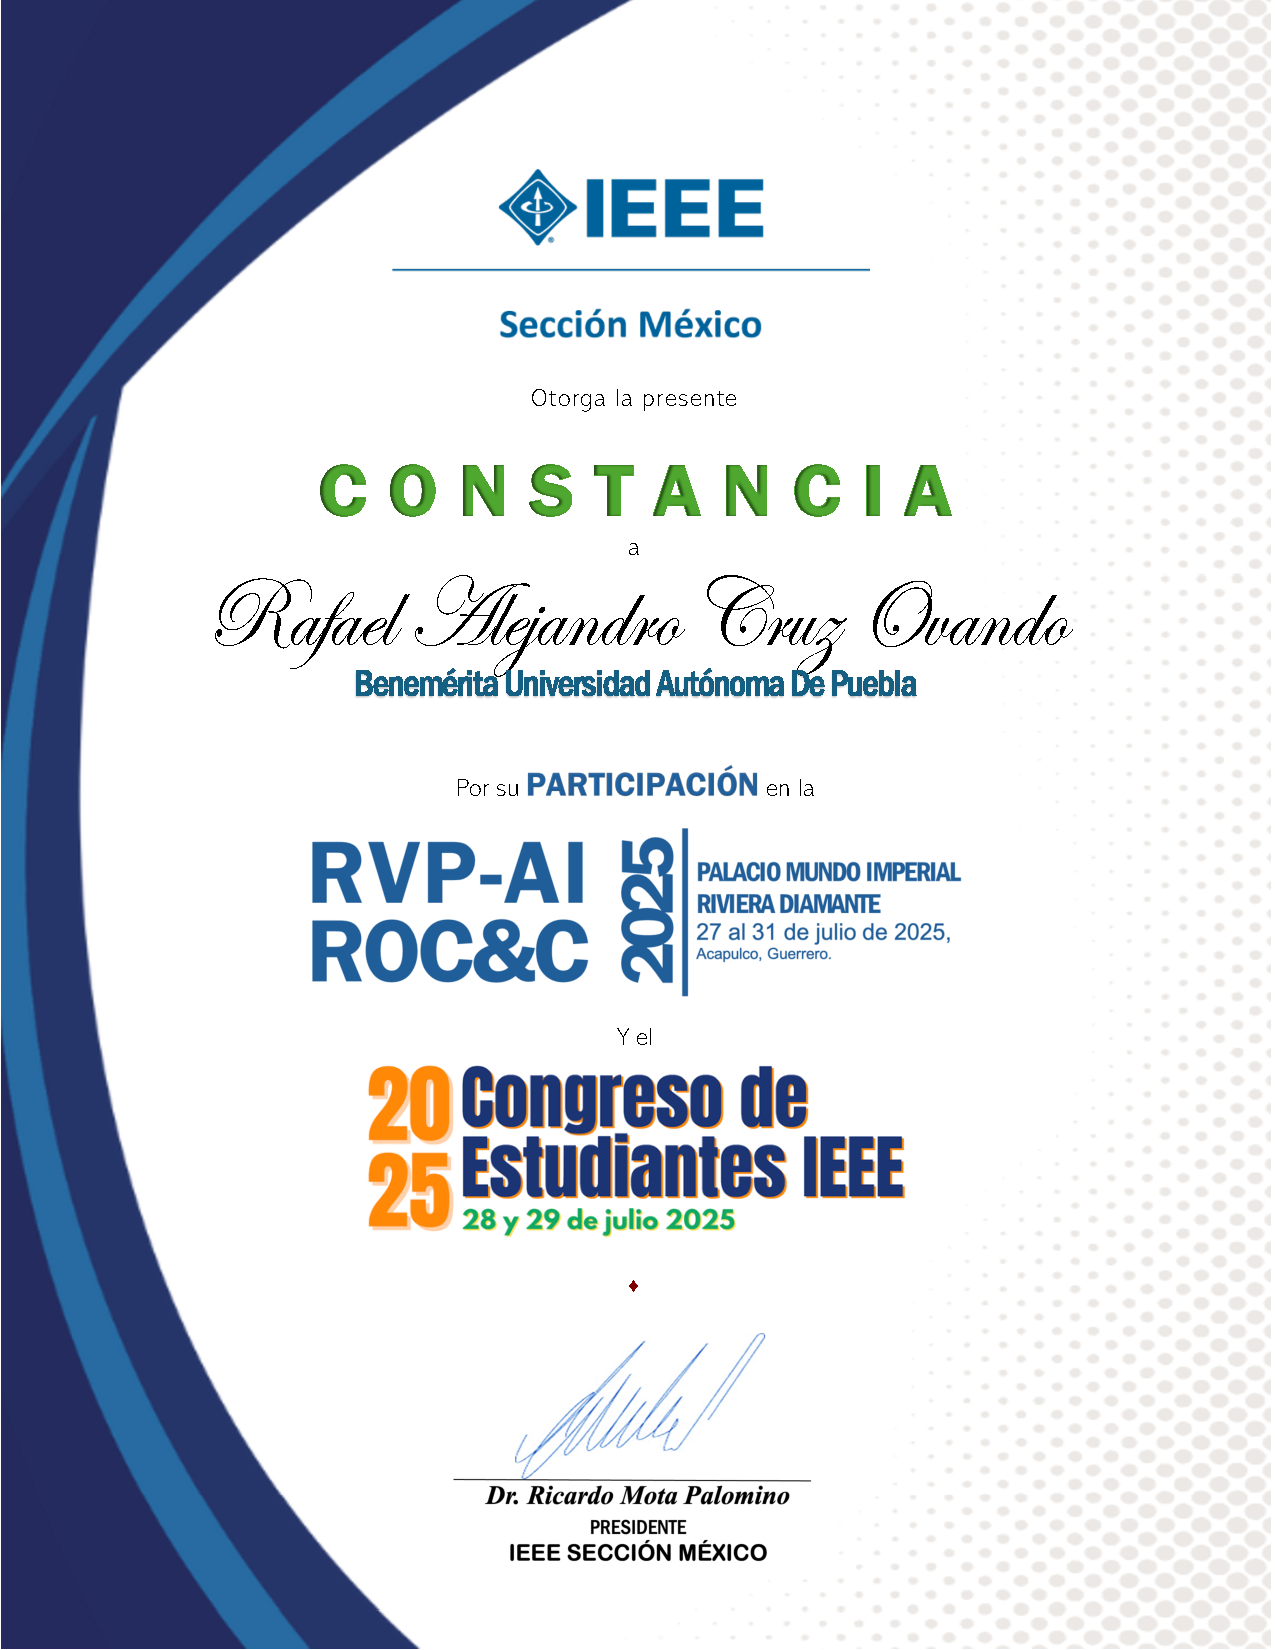
\includepdf[pages=-,pagecommand={\thispagestyle{plain}}]{anexos/constancia_participacion_rafael.pdf}

\section{Reconocimiento - Ponente en Taller de Visión por Computadora}

\textbf{Evento:} Taller ``Visión por Computadora''

\textbf{Fecha:} 17 de septiembre de 2025

\textbf{Lugar:} Facultad de Ciencias de la Electrónica, Benemérita Universidad Autónoma de Puebla

\textbf{Institución organizadora:} Sociedad de Robótica y Automatización (RAS) - IEEE BUAP

\textbf{Tipo de participación:} Ponente del taller

\textbf{Firmante:} Eder Yubaí Hernández Marcelino (Presidente RAS IEEE BUAP)

\textbf{Descripción:} Este reconocimiento se otorga por la participación como ponente en el taller de ``Visión por Computadora'', organizado por la Sociedad de Robótica y Automatización (RAS) del IEEE BUAP. El taller abordó temas de entrenamiento y prueba de redes neuronales convolucionales.

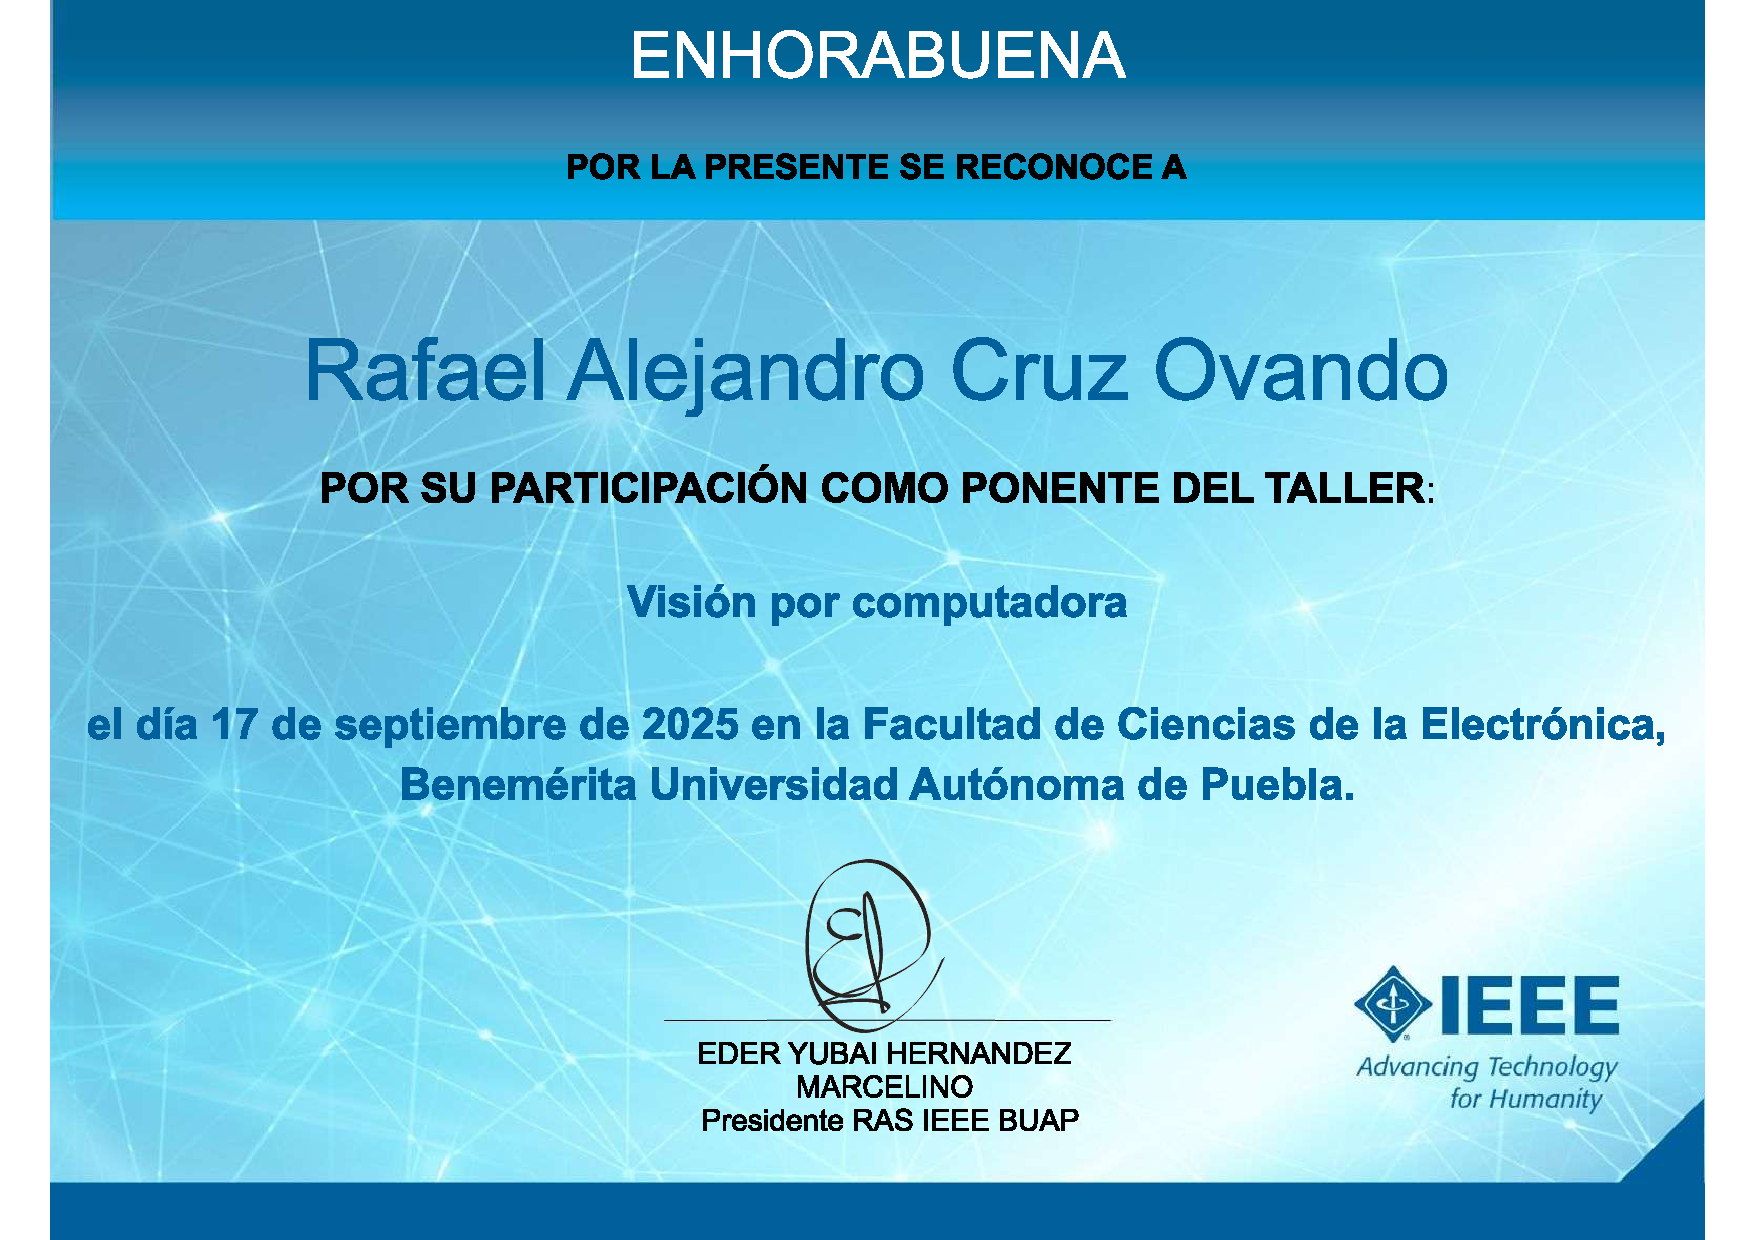
\includepdf[pages=-,pagecommand={\thispagestyle{plain}}]{anexos/reconocimiento_ras_day.pdf}


\newpage
%----------------------------------------------------------------------------------------
%       ANEXO D: CÓDIGO FUENTE
%----------------------------------------------------------------------------------------
\chapter{Código Fuente}
\label{anexo:codigo_fuente}

El código fuente completo del sistema desarrollado en esta tesis está disponible públicamente en un repositorio de GitHub, permitiendo la reproducción de los experimentos y la extensión del trabajo.

\section{Repositorio GitHub}

\textbf{Nombre del proyecto:} Sistema de Normalización Geométrica para Detección de COVID-19 en Radiografías de Tórax. (LungAlignment)

\textbf{URL:} \url{https://github.com/Rhaink/LungAlignment}

\textbf{Lenguaje:} Python 3.12

\textbf{Framework principal:} PyTorch 2.4.1

\textbf{Licencia:} MIT

\section{Contenido del Repositorio}

El repositorio incluye:

\begin{itemize}
    \item Implementación completa de los 4 módulos del sistema:
    \begin{itemize}
        \item Preprocesamiento (CLAHE, SAHS)
        \item Detección de puntos de referencia (ResNet-18 + Coordinate Attention)
        \item Normalización geométrica (GPA, Delaunay, Warping)
        \item Clasificación (ResNet-18 transfer learning)
    \end{itemize}
    \item Configuraciones experimentales validadas (formato JSON)
    \item Scripts de entrenamiento y evaluación reproducibles
    \item Documentación técnica
    \item Tests unitarios
\end{itemize}

\section{Instalación y Uso}

Para reproducir los experimentos:

\begin{verbatim}
# 1. Clonar repositorio
git clone https://github.com/Rhaink/LungAlignment
cd prediccion_warping_clasificacion

# 2. Instalar dependencias
pip install -r requirements.txt

# 3. Ejecutar proceso completo
bash scripts/quickstart_warping.sh
\end{verbatim}

Instrucciones detalladas disponibles en el archivo \texttt{README.md} del repositorio.

\section{Reproducibilidad}

Los resultados reportados en el Capítulo 5 son completamente reproducibles.

\section{Contacto}

Para preguntas o reportar problemas:

\begin{itemize}
    \item \textbf{Issues:} \url{https://github.com/Rhaink/LungAlignment/issues}
    \item \textbf{Email:} co223470443@alm.buap.mx
\end{itemize}


% ============================================================================
% GLOSARIO
% ============================================================================
\newpage
\input{glosario}

\end{document}
